\documentclass{pracamgren}

%\usepackage{color}

\usepackage[T1]{fontenc}
\usepackage{lmodern}

\usepackage[table, svgnames, dvipsnames]{xcolor}
\usepackage{algpseudocode}
\usepackage{algorithm}
\usepackage[framemethod=tikz]{mdframed}
\usepackage{amsmath}
\usepackage{amsfonts}
\usepackage{epsfig}
\usepackage{pstricks}
\usepackage{graphicx}
\usepackage{algorithm}
\usepackage[backend=biber,style=authoryear-comp,sorting=nyt,maxcitenames=2,uniquename=false,uniquelist=false,maxbibnames=5,maxsortnames=1]{biblatex}
\usepackage[font=small,labelfont=bf]{caption}
\usepackage[hidelinks,allcolors=black]{hyperref}
\usepackage{upgreek} 
\usepackage{placeins}
\renewcommand{\arraystretch}{1.1}

\setlength{\parskip}{0pt}

\addbibresource{msc-thesis.bib}

\author{Maciej Manna}

\nralbumu{1065745}

\title{Massively Parallel Pseudo-Spectral DNS and~LES for Particle-Laden Turbulent Flows under Two-Way Momentum Coupling}

\tytul{Masywnie równoległe pseudo-spektralne symulacje DNS i LES przepływów turbulentnych z\,cząstkami przy uwzględnieniu dwustronnego sprzężenia pędu}

\kierunek{computer science}

\opiekun{Dr. hab. Bogdan Rosa \\
Warsaw University of Life Sciences -- SGGW \\
Institute of Information Technology; \\
Institute of Meteorology and Water Management \\ National Research Institute
}

\date{September 2022}

\keywords{obliczeniowa mechanika płynów, przepływ turbulentny, przepływ wielofazowy, krople, mikrofizyka chmur, obliczenia dużej mocy, równania Naviera-Stokesa, homogeniczna izotropowa turbulencja, statystyki zderzeniowe kropel, metoda pseudo-spektralna, bezpośrednia symulacja numeryczna (DNS), metoda dużych wirów (LES), dwustronne sprzeżenie pędu, efekty grawitacyjne}

\keywordsang{computational fluid mechanics, turbulent flow, multiphase flow, droplets, cloud microphysics, high performance computing, Navier-Stokes equations, homogeneous isotropic turbulence, droplet collision statistics, pseudo-spectral method, direct numerical simulation, large-eddy simulation, two-way momentum coupling, gravitational effects}


\begin{document}
\maketitle

\streszczenie{
Przepływy turbulentne z cząstkami fazy rozproszonej zachodzą nieustannie w środowisku naturalnym oraz znajdują liczne zastosowania w procesach przemysłowych.
Ważnym tego przykładem są chmury atmosferyczne, które składają się z ogromnej ilości małych kropel wody i kryształków lodu.
Wyjaśnienie wzajemnego oddziaływania powietrza (płynu) i aerozolu (cząstek) jest istotne w kontekście poznania mechanizmów rządzących powstawaniem i przebiegiem zjawisk atmosferycznych.
Wiedza w tym zakresie jest użyteczna w obszarze meteorologii i służy do opracowywania coraz to bardziej realistycznych modeli powstawania opadu z kropel chmurowych.
To z kolei prowadzi do podniesienia dokładności i sprawdzalności numerycznych prognoz pogody.
Jednym ze sposobów badania przepływów dyspersyjnych są symulacje numeryczne. 
\newline \indent
Powszechnie stosowanym do tego celu narzędziem, zapewniającym wysoką dokładność, są tzw. bezpośrednie symulacje numeryczne (direct numerical simulation, DNS). 
Za pomocą symulacji DNS można pozyskiwać statystyki zderzeniowe cząstek, które to są użyteczne jako parametry w modelach obejmujących większe skale przestrzenne.
Symulacje DNS są~jednak kosztowne obliczeniowo, co ogranicza ich stosowalność do siatek o średnich rozmiarach (${\sim 2048^3}$ węzłów -- przy współcześnie dostępnych zasobach obliczeniowych).
DNS nie pozwalają modelować turbulencji charakteryzowanej wyższymi liczbami Reynoldsa ($R_{\lambda} \sim 10^4$), czyli takiej która obserwowana jest w powietrzu atmosferycznym. \newline \indent
Metoda dużych wirów (large-eddy simulation, LES) stanowi alternatywę dla DNS.
W tej metodzie drobnoskalowa turbulencja nie jest bezpośrednio rozwiązywana, ale jest parametryzowana przy użyciu modelu podskalowego.
Umożliwia to modelowanie przepływów turbulentnych o większej liczbie Reynoldsa przy użyciu siatek o mniejszej liczbie węzłów.
Ograniczenie złożoności obliczeniowej odbywa się jednak kosztem mniejszej precyzji i fizycznej dokładności.
Niniejsza praca stanowi porównanie obu metod (DNS i LES), zarówno w kwestii fizycznej dokładności, jak i wydajności, skupiając się w szczególności na symulacjach z dwustronnym sprzężeniem pędu pomiędzy płynem i cząstkami. 
Zostało wykazane, że LES stanowi obiecującą odpowiedź na ograniczenia DNSu, pomimo pewnych niedokładności wynikających z filtrowania turbulencji w najmniejszych skalach.
Różnice te, w większości przypadków, stają się mniejsze, gdy uwzględni się dwustronne sprzężenie pędu, w szczególności dla cząstek poddanych działaniu grawitacji.
\newline \indent
Przeprowadzone zostały również analizy kosztów obliczeniowych obu metod.
Choć zastosowanie LES zapewnia ogromną oszczędność w obliczeniach związanych z turbulentnym przepływem płynu, to jednak koszt ten znacząco rośnie wraz z liczbą cząstek.
Niezbędna ilość symulowanych cząstek może zaś być duża, gdyż efekty dwustronnego sprzężenia pędu objawiają się wyraźniej w układach z względnie wysokim stosunkiem masy cząstek i płynu (pomiędzy $0.1$~i~$1$).
Obliczenia odnoszące się do dynamiki cząstek stanowią więc bardziej istotne ograniczenie dla LESu niż dla DNSu, gdzie złożoność obliczeń związanych z~płynem jest czynnikiem dominującym.
Ponadto zidentyfikowano i przeanalizowano szereg parametrów, które pośrednio wpływają na czas trwania symulacji, takie jak np. promienie kropel oraz~działanie grawitacji.
Na~koniec przedstawiono także wpływ preferencyjnego koncentrowania się cząstek na wariancję ich rozkładu pomiędzy równolegle wykonywanymi procesami.
Ten czynnik ma~również istotne znaczenie w kontekście całkowitej wydajności symulacji.
}

\renewcommand{\abstractname}{Abstract}
\begin{abstract}
Turbulent fluid flows with dispersed particles are a common occurrence in nature, as~well~as in many technological processes.
An important example of such systems are atmospheric clouds that consist of a huge number of small water droplets and ice crystals suspended in air.
The~understanding of interplay between air (fluid) and aerosol (particles) is crucial for increasing the accuracy and reliability of numerical weather forecasts through more realistic modelling of atmospheric phenomena.
Performing numerical simulations on a fine scale is one way of studying such processes.

Direct numerical simulations (DNS) prove to be a relatively precise tool that is widely used in these studies.
DNS can be used to obtain the particle collision statistics obtained from these simulations may be further utilised as parameterisations for larger-scale models.
These simulations, however, are costly in terms of computational complexity, hence their application is limited to moderate-sized grids ($\sim 2048^3$ nodes, with the computing power of modern supercomputers).
For that reason DNS are not able to resolve turbulence characterised by~higher Reynolds numbers ($R_{\lambda} \sim 10^4$), which is observed in atmospheric air.  

Large-eddy simulations (LES) provide an alternative approach to DNS.
In this method small-scale turbulence is not directly resolved but parameterised using a subgrid-scale model.
This reduces the grid size required to achieve higher Reynolds numbers (and, thus, computational complexity) at the cost of diminished precision and physical fidelity. 
This thesis provides comparison of DNS and LES, both in terms of physical fidelity and performance, focusing primarily on simulations under two-way momentum coupling between the fluid and particles.
LES is shown to be a promising solution to limitations of DNS, even though it~exhibits certain inaccuracies that may be attributed to the filtering of small-scale vortical structures.
These discrepancies, for the most part, become less pronounced when two-way momentum coupling is considered, especially for settling particles.

Furthermore, a broader study of computational costs for both methods is presented.
Even~though LES provides immense performance advantage when it comes to fluid simulation, it~is~highly susceptible to the growing number of individually tracked particles.
The amount of particles that are needed may be considerable, as effects of two-way momentum coupling manifest when particle mass loadings are relatively high (between $0.1$ and $1$).
Thus, computations related to particles are recognised to be a much more significant bottleneck for~LES than for DNS, where the complexity of fluid simulation is the largest concern.
In~addition, several parameters that indirectly influence the execution time are identified and analysed, such as droplet radii or effects of gravity.
Finally, it is shown that the preferential concentration of particles may affect the variance of their distribution between parallel processes and~consequently influence the overall simulation performance.
 
\end{abstract}


\tableofcontents


\chapter*{Acknowledgements}
\addcontentsline{toc}{chapter}{\numberline{}Acknowledgements}
\label{ch:ack}

This thesis was created as part of a project: \emph{Turbulent flow analysis with the dispersion phase -- the impact of two-sided coupling of momentum and gravity on particle motion statistics} of National Science Centre (NCN) -- OPUS14/2017, project no.: UMO-2017/27/B/ST8/00555.

The access to computational resources and supercomputer \emph{Okeanos} used to obtain results presented in this thesis was provided by Interdisciplinary Centre for Mathematical and Computational Modelling (ICM) at Warsaw University (grants: GA73-14, GA84-22, and G87-1145).

\medskip

First and foremost, I would like to thank the supervisor of this thesis and grants mentioned above, Dr. hab. Bogdan Rosa (Warsaw University of Life Sciences -- SGGW, Warsaw; Institute of Meteorology and Water Management -- National Research Institute, Warsaw), for excellent introduction and guidance in the subject matter of the thesis, as well as continuous encouragement and understanding during the process of its creation.
I would also like to express my gratitude to Dr. Sylwester Arabas (Jagiellonian University, Kraków), who introduced me to the modelling of atmospheric clouds and supported in pursuing further involvement in that field, for his valuable comments, as well as aid in administrative affairs.
Furthermore, I would like to acknowledge all creators, maintainers, and developers of the pseudo-spectral solver code, especially Prof. Lian-Ping Wang (University of Delaware; currently Southern University of Science and Technology, Shenzhen) and Dr. hab. Bogdan Rosa, as well as the copyright holder, University of Delaware, for permission to use and modify it in order to obtain results presented in this thesis.
Finally, I would like to thank Prof. Jacek Pozorski (Institute of Fluid Flow Machinery, Polish Academy of Sciences, Gdańsk), as well as all participants of A2S Group Seminar (AGH University of Science and Technology, Kraków) and Seminar on Partial Differential Equations (Jagiellonian University, Kraków) for valuable questions and discussions that helped in shaping the final draft of this thesis. 



\chapter*{Introduction}
\addcontentsline{toc}{chapter}{\numberline{}Introduction}
\label{ch:int}

Turbulence is the phenomenon that accompanies most of the real-world situations where fluid flows are encountered.
Distinction between laminar and turbulent flows is very practical, as the former represents much more organised, layered, and stable fluid motion that is easier to analyse and quantify, while the latter is inherently irregular, and its parameters have to be approached statistically.
Turbulence gives rise to eddies that span wide range of spatial and temporal scales where different dynamical properties of the fluid are most pronounced.
We commonly distinguish three subranges in the entire span of eddy sizes.
There is integral length scale that includes largest eddies containing most of the energy of a system.
Then, we consider inertial subrange, where turbulence kinetic energy is transferred from larger eddies to the smaller ones in a process referred to as the energy cascade.
Finally, we have subrange that consists of smallest eddy sizes, the so-called Kolmogorov microscale, where influence of fluid viscosity is paramount, and where the kinetic energy of slowly vanishing eddies is dissipated into heat.
Such complex behaviour arises due to the nonlinearity of equations governing the fluid motion, which makes turbulent flows famously difficult to study analytically.
Hence, numeric simulations are often employed to model and study these physical phenomena.

Many processes that involve fluid flows, whether laminar or turbulent, are composed of more than one phase.
Here, by phase, we understand regions of the system with the same properties that can be clearly separated by some interface from others.
We refer to such flows as multi-phase, or two-phase, in a common case where the number of considered phases is limited to two.
These phases often are of different states of matter, e.g. gas--liquid for air bubbles flowing in the water pipe, but systems with two immiscible liquids, such as water and crude oil in pipelines, are also studied \parencite{Brauner2003}.
In many cases, one of the phases may be treated as continuous (referred to as the continuous phase, or the carrier fluid), while the other remains in separated chunks.
We refer to such chunks as the disperse phase, and examples may include air bubbles, water droplets, solid particulate matter suspended in a fluid, etc.
Often enough, elements of disperse phase may be approximated as point particles, i.e. material points that are conceptually representing small spheres of given radii, that are considered insoluble and immiscible (that is, they cannot exchange mass with the carrier fluid, suddenly appear, or be destroyed).
Such approximation is especially accurate when disperse phase consists of small droplets or bubbles of one fluid surrounded by another, as the surface tension naturally preserves spherical shape of disperse elements.
Cloud droplets, in particular, remain spherical since the capillary pressure is several orders of magnitude larger than the local fluid shear stress induced by the disturbance flow associated with their motion.
Furthermore, \textcite[Figure 1, therein]{Balachandar2010} point out that for such approximation to be valid, particle response times have to be greater than Kolmogorov time scale of background turbulent flow. 
We shall refer to two-phase flows with disperse phase approximated by point particles as particle-laden.

The modelling of flows that both exhibit turbulent behaviour and include population of particles interacting with that flow gives rise to even more complexity.
As stated by \textcite{Balachandar2010}, ``turbulence and multiphase flows are two of the most challenging topics in fluid mechanics, and when combined they pose a formidable challenge, even in the dilute dispersed regime''.
In spite of that, the number and importance of real-life applications that involve such systems is quite significant, and more than justifies development of effective methods in that domain.
To mention just a few, we may consider some technological, and industrial applications, such as analysis of combustion of liquid fuel aerosols in engines, or combustion of pulverised coal in furnaces \parencite{Zheng2020}, as well as other technologies, including fluidised beds, transport systems, and pollution control \parencite[4-17]{Crowe2012}.
Such systems are also studied in ecology (e.g. transport of pollutants in the atmosphere or sediments in water) and agriculture (efficient spraying of fertilisers).
Finally, the modelling of atmospheric clouds, that essentially are huge collections of small water droplets and ice crystals suspended in often turbulent air, is the backbone of all meteorological and climate science models used for analysis and prediction \parencite{Devenish2012, Grabowski2013}.
In this thesis we shall focus our study of particle-laden turbulent flows on applications in cloud modelling, but general methods presented here are not limited to that particular use case.

The modelling of atmospheric clouds is a broad domain that has to deal with wide range of length scales, where different structures and physical processes are important and have to be directly represented, while others need to be parameterised due to constraints in computing power.
Such tradeoff between computational complexity and physical fidelity of simulations gives rise to the plethora of methods used depending on the respective scale.
Simplified picture of that situation is presented in Figure \ref{fig:atmo-scales}.
At the largest scales we have global climate models (GCM) and global weather models (GWM, e.g. Integrated Forecasting System, Global Forecasting Systems, ICON), where computation domain  often spans the entire Earth ($\sim 10^{7}$~m) and each cell has (horizontal) dimensions ranging from $10$ to $100$ kilometres.
We also consider mesoscale models that are mainly used for weather prediction in smaller domains that usually cover regions, countries, or continents ($\sim 10^{5} \text{--} 10^{6}$ m) and grid spacing is in the order of kilometres.
For instance, maximal resolution of mesoscale model COSMO used for weather forecasting in Poland is $2.8$ km \parencite{Doms2021}.
In this context it is worth adding that a small cloud with a volume of $1 \; \text{km}^3$ may contain $10^{17}$ or more droplets.
Both types of models, due to relatively large grid cell sizes, cannot fully resolve even fairly large cloud structures and depend on a lot of parameterisations.
In the middle ground, we have cloud resolving models (CRM; domain sizes---kilometres, cell sizes---metres) that cannot fully resolve all turbulent scales of air or exactly model behaviour of every droplet, thus necessary parameterisations are employed, such as large-eddy simulations (LES) and super-droplet method \parencite{Arabas2013}.
CRM is commonly employed for research studies focused on the effects of microphysical processes affecting entire clouds, their formation and evolution, precipitation, etc.
For that reason, CRMs are used to refine cloud parameterisations used in GCM and mesoscale models.

\begin{figure}[h]
\centering
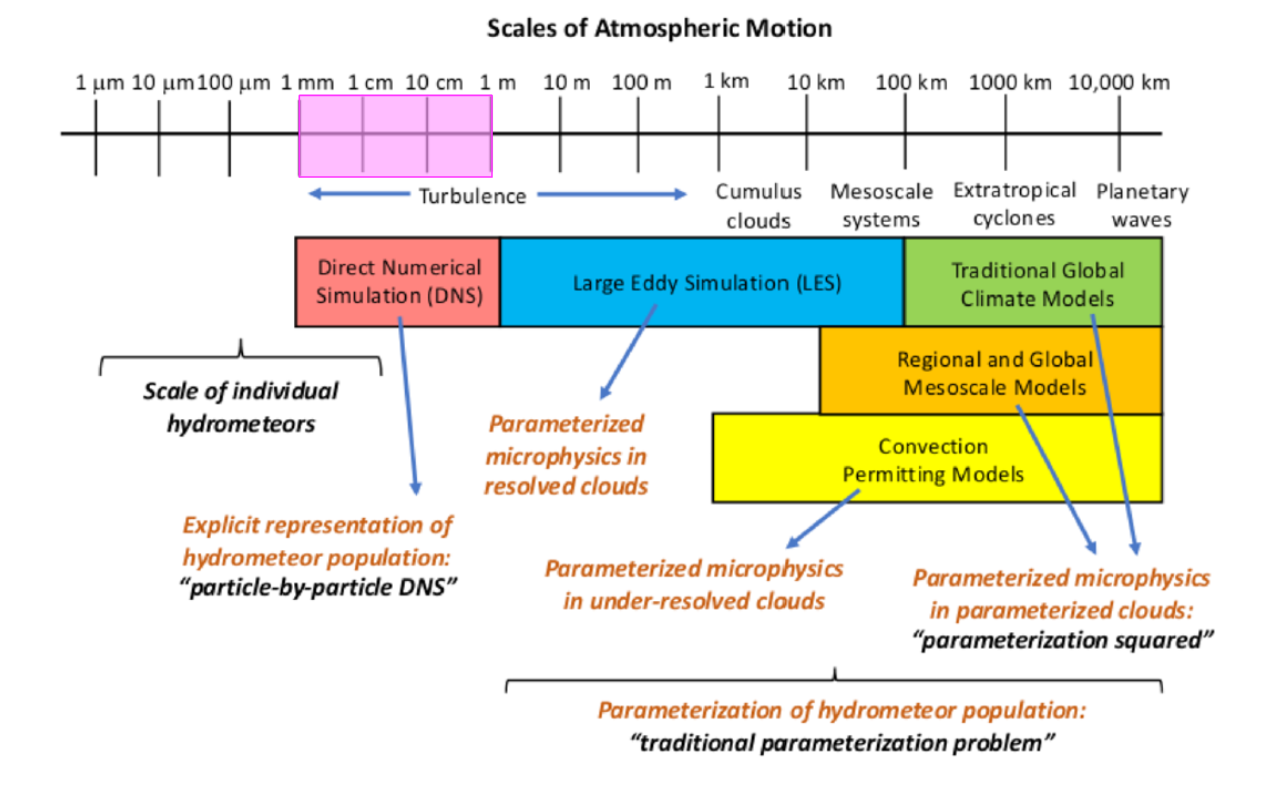
\includegraphics[width=13cm]{figures/0-01_atmo-scales.png}
\caption{
Hierarchy of atmospheric models and the scales of atmospheric motion reproduced from \textcite{Morrison2020} with author's permission.
Coloured rectangles represent types of simulations commonly used when working with respective length scales, and comments emphasise transition from directly resolving most elements of the model (left) to including more and more parameterisations with the increase of scale (right).
Magenta rectangle positioned on the axis was added to emphasise range of scales that corresponds to simulations discussed in this thesis.
}
\label{fig:atmo-scales}
\end{figure}

Finally, we enter scales where point-particle direct numerical simulations (DNS) can be used to obtain more precise picture of small-scale turbulent phenomena that affect cloud microphysics.
These methods allow direct resolution of wide range of turbulent scales, including Kolmogorov microscales, which are estimated to be of the order of 1 mm in Earth's atmosphere.
Also, all particles (droplets) are individually tracked, so that their dynamics and interaction with carrier flow may be directly computed (note, that $1 \, \text{m}^{3}$ of cloudy volume contains, approximately, up to $10^{8}$ droplets).
Due to fine sizes of grid cells required to resolve even the smallest eddies, as well as considerable computational demand of handling large numbers of particles, point-particle DNS are limited to volumes of about $1 \, \text{m}^{3}$ \parencite{Morrison2020}.

Despite these limitations, however, such simulations provide essential backbone to entire hierarchy of models by allowing to study small-scale cloud phenomena and estimate parameters used in cloud resolving models (CRM).
One example of such parameter is the collision kernel that determines rates of collision between droplets of the same or different sizes, and it greatly affects process of droplet growth due to coalescence that is crucial for accurate modelling of precipitation.
Such small domains also justify modelling air turbulence as homogeneous and isotropic.
Even though energy-containing large-scale eddies in atmosphere generate large-scale inhomogeneity and anisotropy, dissipative small-scale eddies work to flatten the inhomogeneities, leading to local homogeneity and isotropy.
This local homogeneity assumption is the basis of most turbulence models \parencite{Matsuda2021}.

There is, however, another important axis which exhibits similar complexity--fidelity tradeoff, and it pertains to the precision of modelling interactions between particles and carrier fluid.
We use Lagrangian approach to track particles, since time microscales associated with the energy dissipation of atmospheric flows and response times of cloud droplets are usually of the same order (i.e. the Stokes number, $St$, is close to $1$, see \cite{Balachandar2009}).
The modelling of interaction between fluid and particles, however, may be limited to one-way momentum coupling (OWC).
It means that particles are transported by the fluid but do not affect its velocity field.
This simplification is valid for dilute systems, where ratio of total mass of particles to total mass of fluid (referred to as the particle mass loading, $\Phi_m$, of the system) is small, usually assumed to be less than $0.1$ (i.e. less than $0.01\%$ by volume for water droplets in air).
Despite that, experiments have shown that presence of particles alters statistics of the carrier fluid flow, e.g. suppresses or enhances the turbulence flow depending on the sizes of particles \parencite{Gore1989}.
Also, recent simulation studies \parencite{Rosa2020} have shown that inclusion of momentum transfer in the other direction, i.e. two-way momentum coupling (TWC), provides a more complete and complex picture of system dynamics, and increase physical fidelity of obtained results, even for relatively dilute systems.
Hence, TWC approach is used here, building upon methods and results from \textcite{Rosa2020,Rosa2022}.
Note, that for very dense systems ($\Phi_m > 1$) it is preferable to also include effects of collisions between particles (four-way momentum coupling), but such conditions are not applicable when considering Earth's atmospheric clouds.
Also, in this context, it is worth to mention alternative methods for modelling interactions between particles, such as simplified representation of many-body aerodynamic interactions \parencite[Hybrid DNS, see][]{Wang2009, Ayala2007} or inclusion of lubrication forces \parencite{Ababaei2021}, however these approaches are beyond the scope of this study.

\smallskip

In this thesis, small-scale simulations of turbulent, particle-laden flows are considered for the purpose of obtaining particle collision statistics, such as previously mentioned collision kernels.
The domain in question is small enough that we can employ direct numerical simulations for the modelling of homogeneous isotropic turbulence (HIT).
For simplicity, the domain is assumed to be box-shaped and uniformly divided into cubic cells in all three dimensions.
Also, periodic boundary conditions are imposed on the domain walls.
As introduced above, the default method applicable for such experiments is point-particle DNS.

Recent studies, however, have shown that direct numerical simulations are close to their limits due to prohibitively large computational costs.
\textcite{Rosa2013,Rosa2016} used grids of up to $1024^3$ nodes, which seems to be the reasonable limit for most studies, although there were studies using even larger grids---e.g. $2048^3$ nodes in \textcite{Ireland2016} and \textcite{Matsuda2021}; for flows without particles grids of size $8192^3$ were used \parencite{Buaria2019} and more recently even up to $12\,288^{3}$ \parencite{Buaria2020}.
It is important to note that grid size is crucial for turbulent flow simulations since it affects the range of spatial scales that can be resolved---from the smallest eddies with sizes close to the spatial grid spacing, to the largest ones of sizes typically about $1/3$ of the computational domain (this limitation is due to a numerical requirement that the correlation of fluid velocity at distances comparable to the domain size must vanish).
Such range between largest and smallest resolvable scales can be expressed using Reynolds numbe, which is commonly interpreted as a measure of magnitude of turbuence.
Examples of values of the Taylor microscale (that is, considering only eddies in inertial subrange) Reynolds number, $R_{\lambda}$, attained in previous high-resolution studies are $R_{\lambda} = 499$ for $1024^3$ grid \parencite{Rosa2013,Rosa2016}; $R_{\lambda} = 597$ \parencite{Ireland2016}, and $R_{\lambda} = 531$ \parencite{Matsuda2021} for $2048^3$ grids; $R_{\lambda} = 650$ for $8192^3$ \parencite{Buaria2019}; and $R_{\lambda} = 1300$ for $12\,288^3$ grid.
It is desirable, however, to attain higher values of $R_{\lambda}$ to simulate conditions that are present in typical atmospheric clouds, where $R_{\lambda}$ is known to attain values between $10^{3}$ and $10^{4}$.
What is more, the increase of the Taylor microscale Reynolds number with the number of grid nodes in one dimension, $N$, is sublinear (comparison of simulation data from various studies shows that $R_{\lambda} \propto N^{2/3}$, see \cite{Wang2009}, Figure 1 therein, which agrees with theoretical estimates for pseudo-spectral method in \cite{Pope2000}, Equation 9.8 therein).
Thus, when we double $N$ we only increase $R_{\lambda}$ by at most $50\% \text{--} 60\%$, while total number of grid nodes, $N^3$, increases by the factor of $8$.
The strategy of increasing grid sizes of DNS to model somewhat wider range of turbulent scales currently faces not only resource limitations, but is also hindered by the diminishing returns in the long run.
This situation calls for an alternative solution.

Large-eddy simulation (LES) is a well-developed method that is commonly used when dealing with length scales specific to CRM simulations \parencite{Guichard2017}.
Its purpose is to allow modelling of highly turbulent environments in larger domains, where directly resolving smallest eddies is infeasible.
The general idea is to directly resolve larger eddies, as in DNS, but replace the direct resolution of the smallest, dissipative turbulent scales with parameterised model, referred to as the subgrid-scale model.
This way smaller grid sizes may be used to obtain statistics of turbulent flow that are comparable to DNS, including the Reynolds number.

LES focuses on directly resolving larger scales of turbulence since they contain most of the energy of the system, and are most effective transporters of conserved properties (\cite[367]{Ferziger2020}; \cite[352]{Pope2000}).
This property is paramount for CRM, but when using simulations to study small-scale phenomena such strategy is not as easily transferable.
Also, it was repeatedly shown that relative motion and preferential concentration of low-inertia particles is governed mainly by small turbulent structures.
Consequently, the collision-coalescence depends on scales of motion that belong to the dissipation subrange of the energy spectrum.
The interest in applying LES method in small-scale experiments used to estimate particle statistics may be limited, but is growing in recent decades \parencite{Fede2006, Jin2010, Rosa2017}, but no comparable studies that also include effects of TWC were performed.
Therefore, it is called for to investigate feasibility of LES in that context, and this thesis aims at providing good starting point for such analyses.

\medskip

The first systematic study using DNS of homogeneous and isotropic turbulence with non-settling particles (i.e. unaffected by gravity) under two-way momentum coupling was performed more than thirty years ago by \textcite{Squires1990}.
It focused on the effects that particles have on carrier flow, especially the modulation of turbulence and changes in energy and dissipation spectra due to varying particle mass loadings.
Their simulations, due to contemporaneous hardware limitations, used small grid sizes ($32^3$ and $64^3$) and thus were limited to $R_{\lambda} = 38$.
In a follow-up study by \textcite{Elghobashi1993} the effect of gravitational settling was considered but the simulations were limited to decaying turbulence.
Other early studies, such as \textcite{Wang1993} and \textcite{Yang1998}, expanded these results to larger meshes but were limited to the one-way momentum coupling.
More importantly, the latter study \parencite{Yang1998} proposed to use LES to achieve higher $R_{\lambda}$ without going beyond hardware limitations.

These earlier studies, however, did not explicitly consider collisional statistics of particles, such as collision kernels, which are main focus of this thesis.
One of the first systematic studies aimed at estimating these parameters using DNS with homogeneous isotropic turbulence model was \textcite{Ayala2008}, and it was motivated by growing interest in the process of droplet growth due to collision-coalescence.
Their simulations included effects of gravity and were performed at different values of the energy dissipation rate.
In another study by \textcite{Wang2008} the main focus was also on collision statistics, but also hydrodynamic interaction between droplets was considered by employing an original method elaborated by \textcite{Ayala2007}.
In both cases, no influence of particles on the fluid flow was taken into account (as in TWC), but their method attempted to model hydrodynamic interactions between particles instead.
An example of earlier TWC study that focused on  particle statistics may be the work of \textcite{Bosse2006}, that shows significant enhancement in the mean settling velocity when two-way coupling is considered. 
Later, these results were extended by \textcite{Monchaux2017} for wider ranges of particle volume loadings, also reporting decrease in particle preferential concentration with increasing mass loading.

Two important features of further studies, at least from the point of view of this thesis, are: (1) inclusion of two-way momentum coupling between fluid and particles, and (2) use of large-eddy simulations in that context.
Most of these, however, used only direct numerical simulations that were limited to one-way momentum coupling.
\textcite{Rosa2013} provides results from simulations spanning wide range of grid sizes (from $N=32$ to $N=1024$), and shows, in practice, diminishing growth of $R_{\lambda}$ with respect to $N$.
It also analysed the influence of different forcing schemes on the estimated particle statistics.
Further studies by \textcite{Onishi2013} and \textcite{Ireland2016} are notable because of relatively large grids used that allowed to obtain higher values of $R_{\lambda}$ ($N=2048$ with $R_{\lambda}=597$, and $N=2000$ with $R_{\lambda} = 527$, respectively).
Work by \textcite{Onishi2013} is also worth mentioning, as instead of pseudo-spectral method it uses finite-difference method, which is considered to be easier to parallelise and adapt to multiprocessor machines.
On that note, of some interest are also recent papers that use Lattice Boltzmann Method to solve underlying homogeneous and isotropic turbulent flow populated by particles tracked using Lagrangian approach \parencite{Ernst2019,Lain2020}.
These studies, however, used only grids of size $128^3$ and since working with highly turbulent flows was not their main goal they were limited to $R_{\lambda} = 20$.
More recent study of \textcite{Matsuda2021} is notable for used grid sizes (up to $2048^3$) and impressive number of particles tracked (up to $1$ billion), as well as interesting measurements of scale-dependent flatness and skewness of particle distribution fields based on wavelets.
Still, these experiments were limited to one-way momentum coupling.

Nonetheless, as already mentioned, it was recent study of \textcite{Rosa2020} that systematically analysed the effects of including two-way momentum coupling on basic statistics of the carrier flow, as well as collision statistics of particles.
Their results show that using TWC significantly affects particle statistics that measure clustering, radial relative velocities, and collision rates, as well as dependence of these statistics on the particle mass loading.
These results were recently complemented by \textcite{Rosa2022}, where simulations covering broader range of grid sizes were performed (up to $1024^3$), and the influence of TWC on average settling velocity of particles was explored as well. 
Still, both of those studies were limited to DNS method only.

On the other hand, first systematic study of using LES method for simulating steady homogeneous isotropic turbulence for carrier fluid in particle-laden systems was performed by \textcite{Fede2006}.
Simulations were performed using finite-volume method on grids with $128^3$ nodes.
Their effort was focused on measuring influence of subgid-scale modelling on the behaviour of heavy inertial particles at collision distances.
In particular, they established that using LES significantly affects particle concentration and collision statistics, as they depend on small-scale motion of carrier fluid.
Their analysis was limited to non-settling particles.
\textcite{Marchioli2008} arrived at similar conclusions, i.e. that filtering velocity field at small-scales leads to inaccuracies in representation of particle segregation and accumulation phenomena in simulations involving wall-bounded flows.
Meanwhile, \textcite{Yang2008} showed that for different particle statistics, such as longtime single-particle dispersion, some effects of LES parameterisation cancel each other, leading to accurate predictions.
More in depth study on the influence of subgrid-scale modelling on preferential concentration of particles, where principal requirements for such models were established, was proposed by \textcite{Pozorski2009}.

Important comprehensive study of impact of subgrid-scale modelling on particle collision statistics in HIT was performed by \textcite{Jin2010}.
They used the pseudo-spectral method for the fluid flow calculations and their realisation of LES (i.e. using spectral eddy viscosity model) matches numerical method used in this thesis.
Their results confirmed adverse effect of LES on the accuracy of particle-pair statistics, as well as established relation between Stokes number, $St$, and sensitivity of these statistics to subgrid-scale modelling.
They concluded that such effects are most noticeable when $St < 3$.
This study involved only non-settling particles.
It was later complemented by \textcite{Rosa2017} that used the same numerical setup but focused on particles affected by gravity.
Their results confirmed previous conclusions regarding limitations of LES to properly represent collisional statistics, such as radial distribution function and radial relative velocity.
They also established influence of subgrid-scale modelling on seemingly single-particle statistics, such as average settling velocity.
All studies mentioned above were limited to one-way momentum coupling.

\smallskip

The natural continuation of aforementioned studies is to analyse the influence of both such extensions applied together in the same simulations.
Thus, more precisely, the topic of this thesis regards simulations of homogeneous isotropic turbulence with inertial particles under two-way momentum coupling, both with and without effects of gravity, for the purpose of estimating their collisional statistics.
Also effects of particles on basic flow statistics shall be discussed.
Both direct numerical simulations (DNS) and large-eddy simulations (LES) are used to obtain results, providing grounds for comparison of both methods.
To the knowledge of the author, it is the first study in this context, where TWC LES simulations are considered.
For the sake of simplicity, all simulations performed as part of this study will use single, moderately-sized grid of $256^3$ nodes for DNS, and $64^3$ for LES, as in \textcite{Jin2010} and \textcite{Rosa2017}.
This study aims to fit into much broader and pressing issue of computational limits that are faced by DNS and establishment of LES as an alternative that opens way to more faithful modelling of atmospheric turbulence.

\smallskip

The comparison between DNS and LES is carried out in two following aspects.

Firstly, the accuracy, or physical fidelity, of LES is analysed.
Establishing exact measures of accuracy for collisional statistics is a challenging task because of experimental constraints, as simultaneous measurement of positions and velocities of large amounts of small droplets faces technical limitations, although considerable advances have been made recently in that field \parencite{Yavuz2018}.
Moreover, homogeneous and isotropic model of turbulence is an idealisation that could not be exactly replicated in actual physical conditions.
For these reasons it is difficult to obtain experimental results for validation, and due to the complexity of the problem at hand, no analytical solutions are available as well.
On the other hand, difficulties in obtaining experimental data makes estimations of these statistics \emph{in silico} even more valuable.
Thus, as in previous studies, the accuracy comparison will mostly focus on qualitative and quantitative differences between results obtained by DNS and LES.
The results of DNS are used as a baseline, under the assumption that this method is thoroughly studied and frequently used, and thus provides accurate estimates of parameters in question.
Hence, results obtained using LES are compared against them, in order to consider feasibility of LES as a workable replacement for DNS.
The further analysis will focus mainly on simulations under two-way momentum coupling.

Secondly, the performance of these two methods will be compared.
The main advantage of LES is its reduced computational cost while attaining similar values of $R_{\lambda}$.
Such claim needs to be thoroughly verified, especially when simulations with particle-laden flows are considered, where computational load not only scales with grid size used to resolve fluid flow but also with the number of individually tracked particles.
That impact is not easy to predict as computations concerning both phases are performed side-by-side in a massively parallel context.
Thus, a series of experiments will be performed to establish possible performance gains provided by LES and whether they can be easily achieved by using the same code architecture and parallelisation strategy as for DNS.

The organisation of this thesis directly follows goals and aspects of analysis outlined above.
The entire text is divided into three chapters.
The first one consists of brief explanation of the numerical method underlining all simulations used to obtain results presented thereafter.
The emphasis is placed on the pseudo-spectral method used for fluid flow simulation, difference between DNS and LES methods, and modelling of interactions between fluid and particles.
In addition, some information on implementation details is given.
Second chapter introduces relevant flow and particle statistics that are being estimated in simulations.
More importantly, the results of simulations will be presented and analysed here in order to compare the physical fidelity and feasibility of LES vs DNS.
Results related to modelling under one-way momentum coupling will be recreated, and validated with respect to previous studies.
Then, results that include the effect of two-way coupling will be presented for both DNS and LES, depending on particle radii, as well as particle mass loading.
In the last chapter, results of performance comparison between DNS and LES shall be presented and discussed.
These will focus on simulation wall-clock times depending on the various parameters of simulations, in order to estimate their influence on the computational cost of the solver code.
Also, more in-depth profiling data shall be presented, as well as analysis of particle distribution in computational subdomains and its impact on the performance of both methods.



\chapter{Numerical Methods}
\label{ch:ch1}

NNN


\chapter{Physical Fidelity of DNS and LES Results}
\label{ch:ch2}

NNN



\chapter{Comparison of DNS and LES Performance}
\label{ch:ch3}

NNN



\chapter*{Conclusions}
\addcontentsline{toc}{chapter}{\numberline{}Conclusions}
\label{ch:end}

NNN


\appendix
\chapter{Pseudo-Spectral Method in Detail}
\label{app:psm}

NNN



\chapter{Effects of Subgrid-Scale Model on Flow Statistics}
\label{app:sgs}

NNN


\chapter{Super-Particle Parametrisations in Simulations under Two-Way Momentum Coupling}
\label{app:spp}

NNN


\addcontentsline{toc}{chapter}{\numberline{}References}
\printbibliography[title=References]

\end{document}
